\documentclass[
  letterpaper,
  DIV=11,
  numbers=noendperiod]{scrartcl}

\usepackage{silence}
\WarningFilter{latex}{Command \showhyphens has changed}

\usepackage{amsmath,amssymb}
\usepackage{xcolor}
\usepackage{graphicx}
\usepackage{longtable}
\usepackage{booktabs}
\usepackage{array}
\usepackage{float}
\usepackage[round]{natbib}
\usepackage{microtype}
\usepackage{etoolbox}
\apptocmd{\thebibliography}{\sloppy}{}{}
\usepackage{xurl}
\usepackage{tabularray}
\usepackage{bookmark}
\IfFileExists{siunitx.sty}{%
  \usepackage{siunitx}%
}{%
  \def\num##1{##1}%
  \def\SI##1##2{##1~##2}%
  \def\percent{\%}%
} 
\emergencystretch=1.5em 

\hypersetup{
  pdftitle={Cultural Matching and the Persistence of Social Ties},
  pdfauthor={Omar Lizardo},
  colorlinks=true,
  linkcolor={blue},
  filecolor={maroon},
  citecolor={blue},
  urlcolor={blue}
}

\title{Cultural Matching and the Persistence of Social Ties}
\author{Omar Lizardo}
\date{\today}

\begin{document}
\maketitle

\begin{abstract}
How does cultural matching shape the evolutionary dynamics of personal networks during major life transitions? While traditional perspectives often view tastes primarily as malleable byproducts of network transmission, we advance an integrative cultural matching framework in which cultural matching actively protects ties from decay. Using longitudinal ego-network data from the \textit{NetSense} study, which tracked college students across eight survey waves, we find that cultural matching---both in broad categorical domains and in specific leisure activities---significantly reduces the hazard of tie decay. Conversely, cultural network opacity, or a lack of mutual cultural knowledge, acts as an independent liability that accelerates tie decay. Crucially, this protection from tie decay through cultural matching is heavily concentrated among subjectively close ties: cultural matching forms an essential interactional core for maintaining close relationships amidst high background churn, whereas weak ties face such a high baseline rate of decay that cultural matching alone cannot sustain them. These findings show how, within high-turnover peer ecologies, individuals draw upon cultural matching as a portable resource to selectively curate and protect their most meaningful social bonds from decay.
\end{abstract}

\newpage
\section{Introduction}\label{introduction}

A central issue in the study of culture and networks concerns the co-evolution of social ties and cultural tastes \citep{lizardo2006, edelmann2014cultural-a77}. Sociological perspectives on taste diffusion often posit that an individual's cultural profile is continuously molded by their current social network configuration \citep{mark1998b, mcpherson2004blau-9fe}. In this view, tastes diffuse across existing homophilous ties, which are themselves structured by socio-demographic similarity \citep{lazarsfeld1954, mcpherson2001, feld2009homophily-595}. Under this network-transmission imagery, tastes are often construed as fluid, network-contingent contents liable to shift as local network configurations evolve \citep{mark2003}. Yet longitudinal research reveals that personal networks are frequently in flux, with ties being formed, renegotiated, and dissolved---particularly during critical life-course transitions such as entry into college, job changes, or relocation \citep{burt2000, wellman1997, kleinbaum2018reorganization-4a1, roy2022turnover, weiss2022life, kempnich2024how, vacchiano2024networked}. This pervasive network turnover raises an important substantive question: if personal networks undergo substantial turbulence during formative transitions, what explains the relative durability of individuals' cultural dispositions, and how do individuals actively deploy these cultural profiles to navigate volatile social ecologies \citep{bourdieu1984, holt1998}?

In this paper, we evaluate the empirical implications of a \textit{cultural matching model} of tie decay within the dynamic setting of an undergraduate cohort. Rather than treating tastes solely as passive by-products of existing networks, we propose that cultural matching serves as an active micro-interactional ``social glue'' that protects network ties from decay amidst high baseline churn \citep{burt2000}. Under this framework, dyadic cultural matching increases protection from tie decay and enhances the cognitive salience of social ties, operating in tandem with structural and dyadic factors such as subjective closeness, spatial propinquity, and tie duration. Using rich longitudinal ego-network panel data from the \textit{NetSense} study over eight survey waves \citep{bahulkar2016analysis-d8b, bahulkar2017co-evolution-d04, hachen2022generators-923}, we track the decay and persistence of non-kin, on-campus peer ties across multiple college-year transitions. This empirical context provides a strategic window into relationship dynamics during emerging adulthood, capturing both the rapid reorganization of networks during the freshman transition and the subsequent consolidation of personal networks as graduation approaches.

Empirically, we examine the cultural matching mechanism along two interrelated dimensions. First, we establish the baseline protective effect of cultural matching---spanning both broad categorical domains and concrete leisure activities---against tie decay. Second, we introduce the concept of ``cultural network opacity''---the degree to which an ego lacks mutual cultural knowledge about an alter's preferences (indicated by substantive ``Don't Know'' reports)---as an independent predictor of tie decay. By evaluating these mechanisms in a discrete-time event history framework, we illuminate how cultural matching operates as an active mechanism protecting ties from decay within dynamic peer environments.

The remainder of this article proceeds as follows. First, we outline the theoretical framework linking cultural matching, structural position, and tie decay during life transitions. Next, we describe the NetSense data and our discrete-time event history modeling strategy. Finally, we present the empirical results and discuss their theoretical implications for the study of homophily, network turnover, and cultural capital.

\section{Theoretical Framework}\label{theoretical-framework}

\subsection{Tastes and Social Networks}\label{tastes-and-social-networks}

The relationship between cultural tastes and social networks has been conceptualized in two contrasting ways. The \textit{network transmission perspective}, drawing on constructural imagery \citep{carley1991}, views tastes as malleable, network-contingent contents \citep{erickson1988, erickson1996, mark1998a, mark2003}. In this view, social ties constitute the pre-existing ``infrastructure'' or ``pipes'' through which cultural practices diffuse \citep{borgatti2005, erickson1996}. Tastes are learned, adopted, and abandoned based on continuous exchange of cultural information and local bandwagon imitation within an actor's immediate ego network \citep{mark2003}. Because personal networks exhibit substantial over-time volatility---with between one and two-thirds of ties turning over annually in most personal networks \citep{morgan1997, suitor1997}---the network transmission perspective implies that individual tastes must exhibit corresponding volatility.

In contrast, the \textit{cultural capital perspective} conceptualizes tastes as highly durable, embodied dispositions acquired via early socialization \citep{bourdieu1984, bourdieu1990, holt1998, childress2019encultured-e58}. Emphasizing the ``interconvertibility'' of different forms of capital \citep{bourdieu1986}, this view sees cultural aptitudes not merely as by-products of ties, but as fundamental resources that help people form and sustain network connections. Here, networks are seen as fleeting structures built and maintained via interactions \citep{dimaggio1987}. Consequently, individuals actively use pre-existing tastes to construct novel relationships or shed culturally incompatible ties, a dynamic formalized in the cultural matching model \citep{lizardo2006, vaisey2010}. In this framework, internalized cultural practices exert an independent causal effect on the formation of social networks because people self-select into ties based on the match between their tastes and those of others \citep{shalizi2011}.

Building on this insight, recent theoretical elaborations specify how matching and influence operate simultaneously as dual mechanisms. For instance, \citet{lewis2018}, building on early work by \citet{lizardo2006} propose a generalized conversion model showing that cultural conversion (general connectivity as a result of having a wide variety of ties) and cultural matching (forming specific ties with others based on cultural matching) operate in tandem, constrained by the local cultural ecology (the distribution of particular tastes and cultural practices in the relevant setting). Crucially in our present study, the degree of cultural matching at the dyadic level fundamentally determines whether relationships are protected from tie decay or instead selectively dissolve over time \citep{martin2006}. If tastes are durable and personal networks are volatile, it is highly likely that tastes serve as \emph{drivers} of network connections rather than being determined exclusively by them. This leads to the concept of \textit{choice homophily} or cultural matching: new social connections are selected and existing connections are maintained based on pre-existing cultural matching \citep{lazarsfeld1954, werner1979}. In other words, socio-demographic homophily may frequently operate as a \emph{by-product} of active contact selection keyed to cultural matching, rather than as an exogenous structural constraint \citep{carley1991, dimaggio1987}.

\subsection{Cultural Matching and Tie Decay}\label{cultural-matching-and-tie-decay}

A major challenge for any newly formed social relationship is what \citet{burt2000}, drawing on \citet{stinchcombe1965}, refers to as the \textit{``liability of newness.''} Newly formed dyadic ties are fragile and exhibit a high baseline hazard of decay (``tie decay''), which steeply declines as a relationship matures and ripens into close friendship. What protects a tie from decay and helps it overcome this liability of newness? While classic network models emphasize structural factors (such as network constraint or multiplexity) and dyadic factors (such as subjective closeness), we propose that \textit{cultural matching} is a vital protective mechanism against tie decay. Rather than merely indicating demographic similarity, cultural matching serves as an active element that helps people establish basic commonalities in outlook. At the micro-level, cultural matching protects ties from decay by reducing interactional friction, generating positive emotional energy during shared rituals \citep{collins2004}, and providing a common cognitive and behavioral baseline that makes the tie more salient and rewarding to maintain \citep{dimaggio1987}.

When ego and alter exhibit cultural matching, they can coordinate behavior with minimal friction. Over time, this cultural matching increases the cognitive salience of the alter, rendering the tie resistant to decay and protecting it from decay in the ego's active network \citep{burt2000}. Therefore, we expect that cultural matching will significantly reduce the hazard of tie decay, net of subjective closeness and structural controls (\textbf{Hypothesis 1}).

\subsection{Cultural Network Opacity}\label{cultural-network-opacity}

If shared cultural knowledge stabilizes ties, then a \textit{lack} of mutual cultural knowledge---\textit{cultural network opacity}---should act as a major, independent mechanism of tie decay. We define cultural network opacity as the degree to which an ego is ignorant of an alter's cultural preferences. It is important to differentiate opacity from mere lack of cultural matching. A cultural mismatch implies that ego and alter know each other's preferences but do not share them. Opacity, in contrast, implies a relational void. When an ego reports ``Don't Know'' regarding an alter's preferences across multiple domains, it signals a substantial lack of interactional investment. Furthermore, it creates a severe cognitive barrier to finding focal points for shared activities. Without a map of the alter's cultural landscape, the ego cannot easily initiate shared rituals or conversations, independently predicting a higher hazard of tie decay \citep{burt2002, wellman1997}. We test both the main effect of cultural network opacity on tie decay and the moderation of the protective effect of cultural matching by opacity.

\subsection{Tie Strength Contingencies}\label{tie-strength-contingencies}

Furthermore, recent research highlights a critical theoretical tension regarding how the effects of cultural matching intersect with tie strength. On the one hand, drawing on the work of \citet{edelmann2014cultural-a77} and \citet{vaisey2010}, one might expect that cultural matching is primarily associated with the maintenance of \textit{strong} ties. In this view, already grounded friendships characterized by subjective closeness require ongoing cultural matching to sustain intimacy over time, making close ties highly sensitive to cultural matching for protection from decay (\textbf{Hypothesis 3a}). 

On the other hand, a competing perspective, drawn from structural network theory, suggests that strong ties are highly resilient due to emotional inertia, multiplexity, and structural embeddedness, making them less dependent on cultural matching for protection from tie decay. Under this view, cultural matching acts as essential scaffolding specifically for \textit{weak} or nascent ties. Weak ties suffer from a high baseline liability of newness \citep{burt2000}; without cultural matching to grease the wheels of interaction and provide focal points for engagement, they rapidly decay. Thus, the protective power of cultural matching against tie decay should be most pronounced for weak ties (\textbf{Hypothesis 3b}). We estimate interaction models to adjudicate between these competing predictions.

\subsection{Summary of Hypotheses}\label{summary-of-hypotheses}

In sum, we evaluate three core hypotheses regarding the role of culture in network evolution. First, reflecting the stabilizing capacity of cultural matching, \textbf{Hypothesis 1} posits that cultural matching significantly reduces the hazard of tie decay. Second, capturing the relational liabilities of mutual cultural ignorance, \textbf{Hypothesis 2} states that cultural network opacity independently increases the hazard of tie decay. Finally, to adjudicate between competing theoretical mechanisms regarding tie strength, we formulate two alternative predictions: \textbf{Hypothesis 3a} anticipates that protection from tie decay through cultural matching is amplified among subjectively close ties, whereas \textbf{Hypothesis 3b} proposes that protection from tie decay through cultural matching is amplified among weak ties to overcome the liability of newness.

\section{Data and Methods}\label{data-and-methods}

Data for this analysis comes from the \textit{NetSense} study \citep{striegel2013lessons-595}, a longitudinal survey of college students conducted at the University of Notre Dame between 2011 and 2015. The study collected extensive panel data on students' social networks, demographic background, and cultural preferences.\footnote{A comprehensive codebook, data dictionary, and repository for the NetSense project are available at \url{https://olizardo.github.io/NetSense-Codebook/}.} We collected information on the cultural habits of ego-alter pairs using both a series of closed-form domain questions and open-ended activity nominations. For the closed-form items, egos were asked to rate both their own and their alters' level of interest across six broad cultural and leisure domains: \textit{music}, \textit{movies}, \textit{books}, \textit{sports}, \textit{games}, and \textit{outdoor activities}. For the open-ended items, respondents freely nominated up to five leisure activities they enjoyed, and then indicated whether their alter also engaged in each nominated activity. Surveys were administered at the start and end of each semester via Qualtrics during the study period. 

\subsection{Study Waves}\label{study-waves}

For this analysis of tie decay, we pool data across adjacent waves to construct a person-period dataset. To isolate peer dynamics, we restrict our sample to reported non-kin, on-campus ties (i.e., alters who are also Notre Dame students). To capture relationship dynamics throughout the college experience, we construct a discrete-time person-period dataset spanning all available adjacent survey waves (Wave 1 through Wave 8). This design allows us to observe tie decay continuously across varying intervals of the students' academic careers, capturing both the initial network churn of freshman year and the consolidation of networks approaching graduation.

\subsection{Measures and Descriptive Statistics}\label{measures}

Tables \ref{tbl-descriptives-cont} and \ref{tbl-descriptives-cat} present summary statistics for all continuous and categorical variables used in our analyses across the $N = 5,584$ dyad-period observations.

\begin{table}
\centering
\begin{talltblr}[         %% tabularray outer open
caption={Descriptive Statistics (Continuous Variables)\label{tbl-descriptives-cont}},
]                     %% tabularray outer close
{                     %% tabularray inner open
colspec={Q[]Q[]Q[]Q[]Q[]},
hline{2}={1-5}{solid, black, 0.05em},
hline{1}={1-5}{solid, black, 0.08em},
hline{6}={1-5}{solid, black, 0.08em},
column{1}={}{halign=l},
column{2-5}={}{halign=r},
}                     %% tabularray inner close
& Mean & SD & Min & Max \\
Closed-Form Matches & \num{1.67} & \num{1.49} & \num{0.00} & \num{6.00} \\
Open-Ended Matches & \num{2.52} & \num{1.34} & \num{0.00} & \num{5.00} \\
Cultural Network Opacity & \num{0.45} & \num{1.13} & \num{0.00} & \num{6.00} \\
Tie Duration (Years) & \num{4.23} & \num{6.21} & \num{0.02} & \num{21.16} \\
\end{talltblr}
\end{table}


\begin{table}[htbp]
\centering
\begin{talltblr}[         %% tabularray outer open
caption={Descriptive Statistics (Categorical Variables)\label{tbl-descriptives-cat}},
]                     %% tabularray outer close
{                     %% tabularray inner open
colspec={Q[]Q[]Q[]Q[]},
hline{2}={1-4}{solid, black, 0.05em},
hline{1}={1-4}{solid, black, 0.08em},
hline{16}={1-4}{solid, black, 0.08em},
column{1,2}={}{halign=l},
column{3,4}={}{halign=r},
}                     %% tabularray inner close
Variable & Category & N & Percent \\
Tie Persisted (Protection from Tie Decay) & 0 (Decayed) & \num{3935} & \num{70.5}\% \\
 & 1 (Persisted) & \num{1649} & \num{29.5}\% \\
Ego Gender Identity & Men & \num{2901} & \num{54.0}\% \\
 & Women & \num{2471} & \num{46.0}\% \\
Alter Gender Identity & Men & \num{2839} & \num{51.0}\% \\
 & Women & \num{2728} & \num{49.0}\% \\
Subjective Closeness & Not Close & \num{565} & \num{10.1}\% \\
 & Somewhat Close & \num{2611} & \num{46.8}\% \\
 & Close & \num{2400} & \num{43.0}\% \\
Interaction Frequency & Weekly & \num{760} & \num{13.6}\% \\
 & Daily & \num{4824} & \num{86.4}\% \\
Race Homophily & Heterophilous & \num{510} & \num{9.1}\% \\
 & Homophilous & \num{1508} & \num{27.0}\% \\
 & Unknown & \num{3566} & \num{63.9}\% \\
\end{talltblr}
\end{table}


\subsubsection{Outcome Variable: Tie Decay}
\emph{Tie Decay}: Network evolution is evaluated through tie decay between adjacent waves. The outcome is measured as a binary indicator taking a value of 1 if a social tie reported by an ego in a baseline wave (e.g., Wave 1) is still present in the subsequent wave (e.g., Wave 2; protected from tie decay), and 0 if the tie has decayed (i.e., the alter is no longer listed in the ego's network). In our analytic sample, \SI{29.5}{\percent} of dyad-periods persist into the subsequent wave, reflecting the substantial baseline rate of tie decay characteristic of collegiate peer networks. To determine tie presence, egos were asked to list the people with whom they interact most frequently, using the following name generator: ``Please list the people with whom you have spent the most time in the last month.'' Egos could nominate up to 20 alters in each wave. This name generator uses what \citep{marin2007simplifying-74e} refers to as the ``interaction'' approach, which is relatively neutral with respect to tie strength \citep{laumann1989boundary-0af}. Other tie characteristics related to strength, such as duration, role relation (e.g., kin versus friend), and subjective closeness, were collected via follow-up name interpreters. 

\subsubsection{Cultural Predictors} 

\emph{Closed-Form Cultural Matching}: A count variable (ranging from 0 to 6; Mean = 1.67, SD = 1.49) indicating the number of closed-form cultural domains in which the ego and alter exhibit cultural matching. Egos were asked to rate their own interest, and their alters' interest across six broad domains: music, movies, books, sports, games, and outdoor activities. The specific survey prompt for egos was: ``How interested are you in the following activities?'' and for alters: ``How interested is this person in the following activities?'' Response categories included ``Very interested,'' ``Somewhat interested,'' and ``Not at all interested.'' A domain was scored as a ``match'' if the ego rated both themselves and their alter identically. Note that the ego's information was collected in a \textit{separate} survey from the ego-network survey (a demographic survey), which dealt with immediate ordering bias and attenuated any cognitive consistency effects.

\emph{Open-Ended Activity Matching}: A count variable (ranging from 0 to 5; Mean = 2.52, SD = 1.34) capturing the degree of cultural matching across specific leisure activity nominations. Egos were asked to freely list up to five leisure activities they enjoyed with the prompt: ``Please list up to 5 specific activities that you enjoy doing in your free time.'' Subsequently, for each alter, the ego was asked to check boxes indicating which of these specific activities the alter also enjoyed, prompted with: ``Which of your favorite activities does this person also enjoy?''

\emph{Cultural network opacity}: A count variable (ranging from 0 to 6; Mean = 0.45, SD = 1.13) measuring the number of cultural domains for which the ego responded ``Don't know'' regarding their alter's preferences. For the closed-form domain questions regarding alters, respondents were provided a fourth response category: ``Don't know.'' While survey researchers often instinctively treat ``Don't know'' responses as missing data to be imputed or dropped, we explicitly operationalize these responses as substantive data. In the context of ego-network surveys, a ``Don't know'' response is not random missingness; rather, it is a direct behavioral measure of relational ignorance (opacity). By retaining and counting these responses, we treat opacity as a distinct structural feature of the dyadic tie.

\subsubsection{Relational and Structural Controls}

\emph{Subjective Closeness}: Measured with the name interpreter, ``How close are you to this person?'' Response categories were ``Not close'' (\SI{10.1}{\percent}), ``Somewhat close'' (\SI{46.8}{\percent}), and ``Very close'' (\SI{43.0}{\percent}). This is treated as a factor variable in the models. As \citet{marsden1984measuring-f62} noted in their classic paper, this item is the most reliable indicator of tie strength \citep{granovetter1973strength-f5f}.

\emph{Relationship Type}: Derived from the role relation name interpreter ``How are you connected to this person?'' We include binary indicators for whether the tie is a \texttt{Friend} (vs. other types) or a \texttt{Roommate/Dormmate} (capturing on-campus structural propinquity).

\emph{Frequency of Interaction}: Measured with the name interpreter, ``How often do you communicate with this person?'' Responses were dichotomized into a \texttt{Daily} contact indicator (\SI{86.4}{\percent}) versus a reference category of \texttt{Weekly} contact (\SI{13.6}{\percent}).

\emph{Tie Duration}: A continuous measure of how long the ego has known the alter (in years; Mean = 4.23 years, SD = 6.21), asked via the name interpreter: ``How long have you known this person?'' We include both the linear and squared terms (\emph{Duration Squared}) to account for nonlinearities in the liability of newness.

\emph{Structural Embeddedness (Common Neighbors / Triadic Closure)}: To account for the collective, group-embedded nature of personal networks and control for triadic closure \citep{granovetter1973strength-f5f, coleman1988}, we construct a dyadic embeddedness metric from the perceived alter-by-alter acquaintance matrix. In each survey wave, respondents evaluated whether their nominated contacts knew one another (``As far as you know, does [Alter Name] know any of your other contacts that are listed below?''). From this dyadic matrix, we compute the number of common neighbors (shared contacts) that Alter $j$ possesses with other alters in ego's network (Mean = 5.43, SD = 4.29; ranging from 0 to 19). Because the ego is tied to every alter in the roster, each reported alter-alter connection directly represents a closed triangle ($\text{Ego} - \text{Alter}_j - \text{Alter}_k$). In our models, this measure is standardized. For wave intervals where the alter-alter matrix was not included (Wave 6), the variable is standardized using a non-parametric wave transition fixed effect to absorb the baseline shift, and sensitivity checks are conducted on the fully measured waves.

\emph{Demographics}: We control for ego's gender identification (\SI{44.3}{\percent} Women, \SI{52.0}{\percent} Men) and perceived (from ego's point of view) alter gender (\SI{48.9}{\percent} Women, \SI{50.8}{\percent} Men), along with a multiplicative interaction term to capture same-gender vs. cross-gender homophily and heterophily (respectively). We also include a measure of \emph{Race Homophily}, constructed by matching the ego's self-reported race to the alter's perceived race (\SI{27.0}{\percent} Homophilous, \SI{9.1}{\percent} Heterophilous, \SI{63.9}{\percent} Unknown alter race).

\emph{Time Period}: Dummy variables for each wave transition interval (Wave 1 to 2, Wave 2 to 3, Wave 3 to 4, Wave 4 to 5, Wave 5 to 6, Wave 6 to 7, Wave 7 to 8) to allow the baseline hazard of tie decay to vary non-parametrically across the entire panel span.

\subsection{Analytical Strategy}\label{analytical-strategy}

Because our data tracks relationships over time and individuals can nominate multiple alters, our data structure consists of dyad-periods nested within egos. To properly analyze tie decay, capture the high baseline volatility of personal networks \citep{cornwell2021tracking, weiss2022life}, and account for right-censoring, we employ a discrete-time event history framework \citep{singer1993s}. Since the outcome variable---whether a tie is protected from decay into the next wave---is binary, we estimate protection from tie decay (the probability of tie persistence given the tie was active in the previous wave) using mixed-effects logistic regression. This modeling strategy allows us to explicitly model the baseline hazard rate of tie decay across each wave transition, isolating the protective effects of cultural matching against this background volatility.

To address the non-independence of observations arising from the clustered nature of the ego-network data (multiple ties per ego), we include random intercepts for egos. This accounts for unobserved, time-invariant individual heterogeneity in the baseline propensity to maintain ties. 

The models take the following general form:
\begin{equation}
\text{logit}(P(Y_{ijt} = 1)) = \beta_0 + \beta_1 X_{ijt} + \beta_2 C_{ijt} + u_i
\end{equation}

where $Y_{ijt}$ is the indicator of protection from tie decay (persistence vs. decay) for ego $i$ and alter $j$ at time $t$, $X_{ijt}$ represents the vector of our core theoretical predictors (cultural matching and cultural network opacity), $C_{ijt}$ is a vector of dyadic and structural control variables (including time period indicators to allow the baseline hazard to vary non-parametrically over waves), and $u_i$ is the ego-specific random intercept, assumed to be normally distributed with mean zero and variance estimated from the data.

All models are estimated via maximum likelihood using the \texttt{glmer} function from the \texttt{lme4} package \citep{bates2015} in \textsf{R} \citep{Rmanual}. In models that interact subjective closeness with our cultural variables, we calculate and plot predicted probabilities to facilitate the interpretation of the non-linear interaction terms \citep{mize2019best}.

\section{Results}\label{results}

We present our findings in three stages. First, we examine the baseline main effects of cultural matching and opacity on protection from tie decay. Second, we test the competing moderation predictions (Hypotheses 3a and 3b) by interacting our matching variables with subjective closeness. Finally, we evaluate the consistency of our findings using ego fixed-effects (conditional logit) models.

\subsection{Main Effects: Matching and Embeddedness}\label{main-effects}

Table \ref{tbl-models} presents the odds ratios from a series of mixed-effects logistic regression models predicting protection from tie decay. As standard network theory would predict, ties that are subjectively closer ($OR = 2.39, p < 0.001$ for ``Close'' ties in Model 1) are significantly more protected from tie decay. Interestingly, having daily contact ($OR = 1.12, p > 0.05$) does not reach conventional significance levels when adjusting for closeness and other controls in this sample.

Building on this structural baseline, Model 1 shows that \textit{closed-form cultural matching} significantly protects ties from decay. For each additional broad cultural domain exhibiting cultural matching, the odds of protection from tie decay increase by \SI{9.6}{\percent} ($OR = 1.10, p < 0.01$), net of controls.

In Model 2, we introduce \textit{open-ended activity matching}. Cultural matching in specific leisure activities provides additive protective value against tie decay: each shared activity increases protection from tie decay by \SI{8.0}{\percent} ($OR = 1.08, p < 0.05$). When both are included, closed-form cultural matching remains significant ($OR = 1.08, p < 0.05$), indicating that specific activity matching provides protective value beyond broad domain matching.

Model 3 tests the independent main effect of \textit{cultural network opacity}---measured as the number of domains in which the ego reported ``Don't Know'' regarding their alter's preferences. Opacity predicts a \SI{5.3}{\percent} increase in the hazard of tie decay per unknown domain ($OR = 0.95$ for protection from decay). However, this main effect is not statistically significant at the conventional level ($p > 0.05$) when adjusting for both closed-form and open-ended cultural matching simultaneously. The attenuation of this coefficient in the pooled mixed-effects model is likely due to the built-in, between-person correlation between reporting ``Don't Know'' and having fewer known cultural matches. However, as we will show in the interaction models and the fixed-effects sensitivity check below, opacity remains a significant liability in specific relational contexts.

Finally, Model 4 introduces \textit{structural embeddedness}---the standardized count of common neighbors (shared alter contacts) that an alter possesses within ego's nominated network. Consistent with triadic closure and dynamic Simmelian tie arguments \citep{krackhardt2007heider-29f}, having shared network contacts strongly and significantly protects ties from decay ($OR = 1.12, p < 0.05$): each standard deviation increase in the number of common alter contacts increases protection from tie decay by \SI{12.2}{\percent}. Crucially, controlling for structural embeddedness does not eliminate the independent contribution of cultural matching. Both open-ended activity matching ($OR = 1.07, p < 0.05$) and closed-form cultural matching ($OR = 1.07, p = 0.057$) maintain their positive protective associations against tie decay. This shows that dyadic cultural matching is not an artifact of being embedded in dense peer cliques; rather, cultural matching and triadic structure operate as complementary, parallel anchors protecting ties from decay. Supplementary tests interacting cultural matching with structural embeddedness revealed no significant moderation ($p = 0.65$), indicating that cultural matching protects ties from decay across both structurally peripheral and densely embedded relationships.

To contextualize these coefficients, Figure \ref{fig-combined} plots the average marginal effect of each core theoretical variable on the probability of protection from tie decay. Across the board, cultural matching serves as a protective mechanism against tie decay (positive estimates), whereas cultural network opacity accelerates tie decay (negative estimates).

\begin{table}[htbp]
\centering
\begin{talltblr}[         %% tabularray outer open
caption={Odds Ratios for Tie Persistence (Main Effects Models)\label{tbl-models}},
note{}={+ p \num{< 0.1}, * p \num{< 0.05}, ** p \num{< 0.01}, *** p \num{< 0.001}},
note{ }={Note: All models control for ego and alter gender, non-linear tie duration, and baseline hazard variations across all 7 wave transitions (coefficients omitted for space). Random intercepts for egos are included.},
]                     %% tabularray outer close
{                     %% tabularray inner open
width=\linewidth,
colspec={X[2.5,l] X[1,c] X[1,c] X[1,c] X[1.1,c]},
row{odd}={rowsep=0.5pt},
row{even}={rowsep=0.5pt},
hline{2}={1-5}{solid, black, 0.05em},
hline{26}={1-5}{solid, black, 0.05em},
hline{1}={1-5}{solid, black, 0.08em},
hline{29}={1-5}{solid, black, 0.08em},
}                     %% tabularray inner close
 & {Model 1\\Closed} & {Model 2\\+ Open} & {Model 3\\+ Opacity} & {Model 4\\+ Embed.} \\
Closed-Form Matches & \num{1.096}** & \num{1.083}* & \num{1.070}* & \num{1.067}+ \\
 & (\num{0.035}) & (\num{0.035}) & (\num{0.036}) & (\num{0.036}) \\
Open-Ended Matches &  & \num{1.080}* & \num{1.076}* & \num{1.071}* \\
 &  & (\num{0.034}) & (\num{0.034}) & (\num{0.033}) \\
Network Opacity &  &  & \num{0.947} & \num{0.952} \\
 &  &  & (\num{0.038}) & (\num{0.038}) \\
Structural Embeddedness (Common Alters) &  &  &  & \num{1.122}* \\
 &  &  &  & (\num{0.050}) \\
Subjective Closeness: Somewhat & \num{1.440}** & \num{1.388}* & \num{1.368}* & \num{1.342}* \\
 & (\num{0.203}) & (\num{0.197}) & (\num{0.195}) & (\num{0.191}) \\
Subjective Closeness: Close & \num{2.388}*** & \num{2.244}*** & \num{2.188}*** & \num{2.097}*** \\
 & (\num{0.359}) & (\num{0.342}) & (\num{0.336}) & (\num{0.324}) \\
Roommate/Dormmate & \num{0.788} & \num{0.787} & \num{0.783} & \num{0.791} \\
 & (\num{0.195}) & (\num{0.194}) & (\num{0.194}) & (\num{0.197}) \\
Friend & \num{0.714} & \num{0.705} & \num{0.706} & \num{0.712} \\
 & (\num{0.175}) & (\num{0.173}) & (\num{0.174}) & (\num{0.177}) \\
Frequency: Daily (vs Weekly) & \num{1.119} & \num{1.107} & \num{1.085} & \num{1.081} \\
 & (\num{0.146}) & (\num{0.145}) & (\num{0.143}) & (\num{0.143}) \\
Race Homophily: Same Race & \num{0.950} & \num{0.944} & \num{0.935} & \num{0.932} \\
 & (\num{0.122}) & (\num{0.122}) & (\num{0.121}) & (\num{0.120}) \\
Tie Duration (Scaled) & \num{0.796} & \num{0.790} & \num{0.768} & \num{0.740} \\
 & (\num{0.183}) & (\num{0.182}) & (\num{0.178}) & (\num{0.172}) \\
Tie Duration Sq (Scaled) & \num{1.238} & \num{1.262} & \num{1.288} & \num{1.339} \\
 & (\num{0.303}) & (\num{0.309}) & (\num{0.317}) & (\num{0.331}) \\
Num.Obs. & \num{5349} & \num{5349} & \num{5349} & \num{5349} \\
AIC & \num{5147.9} & \num{5143.6} & \num{5143.7} & \num{5139.0} \\
BIC & \num{5273.0} & \num{5275.3} & \num{5282.0} & \num{5283.8} \\
\end{talltblr}
\end{table}



\subsection{Moderation by Subjective Closeness}\label{moderation-by-closeness}

While the main effects show that cultural matching generally protects ties from decaying, we next assess whether the protective effect is observed across all relationship types. To do so, we estimated auxiliary interaction models (not shown in the tables but visualized using predicted probabilities) to test whether the protective effects of cultural matching and the detrimental effects of cultural network opacity are moderated by baseline subjective closeness. Because interaction terms in logistic models can be opaque due to the non-linear link function, we visualize this critical interaction to make the core finding directly interpretable. Figure \ref{fig-closeness-interactions} plots the average marginal effects of our three cultural variables across ties rated as ``Not Close,'' ``Somewhat Close,'' and ``Close.''

The results reveal a structured asymmetry in how cultural matching and cultural network opacity protect ties from decay conditioned on tie strength. We find a strong interaction for both closed-form cultural matching and cultural network opacity, but little interaction for open-ended activity matching. For broad, closed-form cultural matching and network opacity, the predictive slopes (marginal effects) are steepest and most significant for \textit{strong} ties (those rated ``Close''). For these essential relationships, an increase in cultural matching substantially increases the predicted probability of protection from tie decay. Correspondingly, cultural network opacity has its most severe, statistically significant penalty precisely on these same strong ties: a lack of mutual cultural knowledge significantly accelerates their decay for ties that are rated as subjectively close. Conversely, for weak ties (those rated ``Not Close''), the marginal effects for both closed-form cultural matching and opacity are relatively flat, indicating an intrinsic vulnerability to tie decay regardless of cultural matching or opacity in these broad domains.

This interaction suggests that cultural matching and mutual cultural knowledge constitute the substantive ``core'' of deep, institutionalized friendships, requiring ongoing cultural matching to protect them from decay. Weak ties, on the other hand, are fleeting and superficial; their baseline hazard of decay is so high that cultural matching does little to prevent their decay. In contrast, the protective effect of specific, open-ended activity matching operates more uniformly across relationships of all strengths, providing a consistent anchor protecting ties from decay, whether the tie is new or well-established.

\subsection{Robustness Check: Ego Fixed-Effects}\label{robustness-check}

To confirm that our findings are not artifacts of our primary mixed-effects specification, we estimated an Ego Fixed-Effects model using conditional logistic regression \citep{graubard2011conditional-502}. The results are shown in Table \ref{tbl-robustness-models}. By stratifying the likelihood function by ego, this approach leverages only within-ego variance---comparing the alters a single ego retains with those it drops. This more stringent test more effectively isolates dyadic tie characteristics from unobserved individual baseline differences (e.g., an ego's baseline sociability, introversion, or general propensity to use the ``Don't Know'' survey option). 

As shown in the table, the fixed-effects models yield results that are substantively equivalent to those obtained using our random-effects main models. Closed-form cultural matching ($OR = 1.05, p < 0.10$) and open-ended activity matching ($OR = 1.06, p < 0.05$) remain positive predictors of protection against tie decay, with odds ratios very close in magnitude to those in the baseline models. Crucially, in this strict within-ego specification, \textit{cultural network opacity} emerges as a highly significant accelerator of tie decay ($OR = 0.92, p < 0.01$ for protection from decay), reducing protection from tie decay by \SI{8.2}{\percent} per unknown domain. This confirms that while opacity may correlate with overall cultural matching rates across individuals, \textit{within} an individual's personal network, a lack of cultural knowledge about a specific alter is a powerful, independent signal of tie decay. The structural controls---such as being ``Close'' ($OR = 1.99, p < 0.001$)---also maintain their consistent associations with the baseline hazard of tie decay, although the structural embeddedness of the tie is no longer a statistically significant predictor of tie decay at conventional levels.

To better assess the magnitude of these within-ego relationships, Figure \ref{fig-fe-predictions} plots the predicted probability of protection against tie decay across observed values of closed-form cultural matching, open-ended activity matching, and cultural network opacity, conditional on ego fixed effects. Across an individual's personal network, increasing closed-form cultural matching from 0 to 6 domain matches increases the predicted probability of tie persistence from \SI{29.8}{\percent} to \SI{34.4}{\percent}, while increasing open-ended activity matching from 0 to 5 shared activities elevates persistence from \SI{28.7}{\percent} to \SI{33.4}{\percent}. In contrast, cultural network opacity imposes a substantial penalty on tie durability within personal networks: increasing the number of unknown domains from 0 to 6 reduces the predicted probability of protection from tie decay from \SI{31.7}{\percent} to \SI{23.7}{\percent}, representing an \SI{8.0}{\percent} decline in persistence. This confirms that even after purging all between-ego sorting, selection biases, and stable individual traits, cultural matching and opacity powerfully govern the decay of social ties.

\begin{table}[htbp]
\centering
\begin{talltblr}[         %% tabularray outer open
caption={Sensitivity Models: Absorbing First Dissolution and Ego Fixed-Effects\label{tbl-robustness-models}},
note{}={+ p \num{< 0.1}, * p \num{< 0.05}, ** p \num{< 0.01}, *** p \num{< 0.001}},
note{ }={Note: Model 1 restricts follow-up strictly to the initial continuous tie spell until first tie decay or censoring, excluding all subsequent recurrent/rekindled spells. Model 2 stratifies the likelihood by ego (conditional logit), isolating within-ego variation. Both models adjust for alter gender and wave transition fixed effects; Model 1 also includes ego gender and an ego random intercept.},
]                     %% tabularray outer close
{                     %% tabularray inner open
width=\linewidth,
colspec={X[2.5,l] X[1.2,c] X[1.2,c]},
row{odd}={rowsep=0.5pt},
row{even}={rowsep=0.5pt},
hline{2}={1-3}{solid, black, 0.05em},
hline{26}={1-3}{solid, black, 0.05em},
hline{1}={1-3}{solid, black, 0.08em},
hline{29}={1-3}{solid, black, 0.08em},
column{2-3}={}{halign=c},
column{1}={}{halign=l},
}                     %% tabularray inner close
 & Absorbing First Decay & Ego FE (clogit) \\
Closed-Form Matches & \num{1.086}* & \num{1.046}+ \\
 & (\num{0.041}) & (\num{0.027}) \\
Open-Ended Matches & \num{1.038} & \num{1.056}* \\
 & (\num{0.036}) & (\num{0.025}) \\
Network Opacity & \num{0.963} & \num{0.920}** \\
 & (\num{0.042}) & (\num{0.029}) \\
Structural Embeddedness (Common Alters) & \num{1.120}* & \num{1.055} \\
 & (\num{0.055}) & (\num{0.036}) \\
Subjective Closeness: Somewhat & \num{1.254} & \num{1.409}** \\
 & (\num{0.191}) & (\num{0.155}) \\
Subjective Closeness: Close & \num{2.002}*** & \num{1.949}*** \\
 & (\num{0.336}) & (\num{0.233}) \\
Roommate/Dormmate & \num{0.753} & \num{0.810} \\
 & (\num{0.201}) & (\num{0.149}) \\
Friend & \num{0.751} & \num{0.806} \\
 & (\num{0.196}) & (\num{0.149}) \\
Frequency: Daily (vs Weekly) & \num{1.154} & \num{1.078} \\
 & (\num{0.185}) & (\num{0.096}) \\
Race Homophily: Same Race & \num{1.030} & \num{0.926} \\
 & (\num{0.151}) & (\num{0.081}) \\
Tie Duration (Scaled) & \num{0.759} & \num{0.820} \\
 & (\num{0.187}) & (\num{0.146}) \\
Tie Duration Sq (Scaled) & \num{1.304} & \num{1.202} \\
 & (\num{0.346}) & (\num{0.220}) \\
Num.Obs. & \num{4522} & \num{1640} \\
AIC & \num{4209.0} & \num{10669.8} \\
BIC & \num{4350.2} & \num{10777.8} \\
\end{talltblr}
\end{table}


\section{Discussion}\label{discussion}

\subsection{Summary of Key Results}\label{summary-of-key-results}
In this paper, we sought to address a central issue in the study of culture and networks: how does cultural matching shape the evolutionary dynamics of personal networks? Using longitudinal ego-network data from the \textit{NetSense} study, we evaluated the empirical implications of a cultural matching model of tie decay. Our results provide consistent evidence that cultural matching is an important mechanism protecting social ties from decay \citep{burt2000}. Specifically, both broad, closed-form cultural matching and specific, open-ended activity matching independently reduce the hazard of tie decay, even after controlling for dyadic structural embeddedness (triadic closure with other alters). While structural embeddedness itself strongly protects against tie decay ($OR = 1.12, p < 0.05$), it does not displace cultural matching. Furthermore, we identified cultural network opacity---the lack of mutual cultural knowledge---as an independent relational liability that accelerates tie decay. Crucially, we found that protection from tie decay through closed-form cultural matching and the accelerating effect of cultural network opacity are most pronounced among strong ties. For these subjectively close relationships, cultural matching acts as a vital core protecting ties from decay, whereas weak ties appear so fleeting that their baseline hazard of decay is high regardless of cultural matching in these domains. In contrast, the protective effect of specific, open-ended activity matching against tie decay remains consistent across both weak and strong ties.

\subsection{Limitations and Suggestions for Future Work}\label{limitations-and-future-work}
Despite these promising findings, several limitations point toward fruitful avenues for future research. First, regarding operationalization and measurement constraints, the current operationalization aggregates cultural matching across broad domains of lifestyle and taste. Future research could further disaggregate these domains to examine whether high-status cultural genres (e.g., classical music, highbrow literature) confer distinct relational advantages compared to widely popular or subcultural domains \citep{dimaggio1987}. In addition, while our measures focus primarily on positive cultural matching and lack of knowledge (opacity), future work should systematically investigate the role of shared cultural \textit{dislikes} and mutual distastes as distinct symbolic boundaries in tie decay.

Second, our network measures capture the \textit{ego-perceived} relational landscape. While egocentric network data are uniquely suited for measuring an actor's cognitive orientation, subjective closeness, and perceived cultural knowledge about their alters, they capture only one side of the dyad. In non-reciprocated or unidirectional ties, relational orientations may be asymmetric, reflecting underlying differences in social status, popularity, or aspirational connection. In such cases, an ego may actively work to maintain a culturally matched tie with a higher-status peer even if the alter does not reciprocate the nomination. Although our ego fixed-effects and dyadic controls account for an ego's general nomination patterns, future sociocentric investigations with complete dyadic reciprocity data can formally evaluate how cultural matching interacts with status differentials and reciprocal confirmation.

Third, regarding threats to causal inference, contextual confounding, and dynamic feedback loops, while our discrete-time event history framework provides a rigorous foundation for modeling the hazard of tie decay net of unobserved heterogeneity, future investigations with continuous digital trace streams would benefit from estimating stochastic actor-oriented models (SAOMs) or continuous-time network dynamics \citep{hachen2022generators-923}. Such models can simultaneously estimate the reciprocal, co-evolutionary processes through which social ties induce taste convergence (influence) and pre-existing cultural dispositions guide tie selection and pruning (selection), while also accounting for unmeasured environmental opportunity structures such as shared course schedules or common extracurricular affiliations.

Fourth, an important question concerns the \textit{temporal horizon} of cultural matching beyond the collegiate context. Our panel follows students through their undergraduate trajectory across semester intervals, capturing the critical period when campus ties are actively formed and pruned. However, a compelling open question is whether cultural matching continues to sustain social ties across major post-collegiate life transitions---such as graduation, geographic dispersal, labor market entry, and family formation. When individuals no longer share the daily scaffolding of an institutional campus environment, does deep cultural matching provide the necessary conversational and ritual currency to protect distant ties from decay across decades? Alternatively, do enduring collegiate ties persist primarily through accumulated relational history and institutional memory, rendering cultural matching less decisive once physical co-presence ends? Future long-term multi-decade panel studies will be vital for determining the life-course boundaries of cultural matching.

Finally, our empirical focus on a college-age cohort during emerging adulthood delineates specific institutional scope conditions for our claims. The transition to college represents a unique developmental and institutional ecology characterized by high baseline network churn, rapid relational renegotiation, and geographic concentration \citep{mcfarland2014network-735}. While this setting provides an ideal testing ground for observing tie decay and protection from decay in real time, future research should examine whether cultural matching operates similarly to protect ties from decay across different life stages and institutional domains. In particular, comparative studies in workplace organizations, civic associations, or among older adults \citep{cornwell2008social-257} could shed light on how the capacity of cultural matching to protect against tie decay varies across differing levels of structural constraint.

\subsection{Implications: Cultural Capital and Relational Maintenance}\label{implications}
These findings carry significant theoretical implications for our understanding of the relationship between tastes and networks, particularly regarding the role of tie strength. Our results heavily favor the empirical implications of the strong-tie matching prediction (\textbf{Hypothesis 3a}) over the weak-tie scaffolding prediction (\textbf{Hypothesis 3b}). Aligning with previous research \citep{edelmann2014cultural-a77, vaisey2010}, our longitudinal event history framework reveals that emerging friendships require ongoing cultural matching to sustain intimacy and prevent tie decay. It is the \textit{strong} ties that are highly sensitive to cultural matching and opacity. Weak ties, suffering from a high liability of newness, rapidly decay with or without cultural matching. These results extend recent observations in life course and network research showing that while significant network turnover is a ubiquitous feature of critical life transitions, individuals actively curate their core networks to maintain stable, supportive ties \citep{roy2022turnover, weiss2022life, kempnich2024how, vacchiano2024networked}. More broadly, our findings challenge the assumption of the pure network-transmission perspective, which treats cultural tastes as merely fluid by-products of existing social ties \citep{mark2003}. Instead, our findings align more closely with the cultural capital perspective \citep{bourdieu1984}, suggesting that tastes function as durable, portable resources that individuals actively use to select, maintain, and discard social relationships. 

Returning to the puzzle posed in the introduction---how do we account for durable cultural profiles in the face of volatile networks \citep{bourdieu1984, holt1998}---our results help to close the loop. If persons use relatively stable cultural dispositions to selectively maintain their networks, it suggests that cultural capital is not merely a passive status marker or a ``thin'' effluvium of network position. Rather, it is an active navigational tool for managing social environments. People churn through weak ties at a high baseline rate, but they rely on their durable cultural compass to actively curate and protect the core relationships that matter from decay.

Furthermore, our findings speak directly to the classic distinction between choice homophily and induced homophily \citep{mcpherson2001}. If cultural matching actively prevents tie decay and opacity accelerates it, then a substantial portion of the observed homophily in established social networks is likely due to selective protection against tie decay (choice homophily) rather than pure structural constraint or network-induced adaptation \citep{lizardo2006, lewis2018}. By protecting culturally matched ties from decay and shedding incompatible ones over time, networks become homophilous through an active evolutionary sorting process.

In this paper, we conceptualize cultural matching as the essential structural core of close relationships. While early network theories emphasized structural constraints or multiplexity \citep{burt2000}, our findings suggest that cultural matching is what protects close relationships from decay. In the absence of mutual cultural knowledge (high opacity), even subjectively close ties face a higher hazard of decay. This developmental view of networks helps reconcile the volatility of personal networks with the relative stability of individual cultural profiles.

Beyond network theory, these findings carry practical implications for institutions aiming to foster social cohesion. For university administrators and community organizers seeking to reduce social isolation, our results underscore that mere proximity or shared structural affiliations are insufficient to sustain durable relationships. Facilitating environments where individuals can discover and activate cultural matching---from niche clubs to diverse recreational programs---may be essential for transforming fleeting initial encounters into resilient, long-term support networks.

\newpage
\begin{figure}[htbp]
\centering
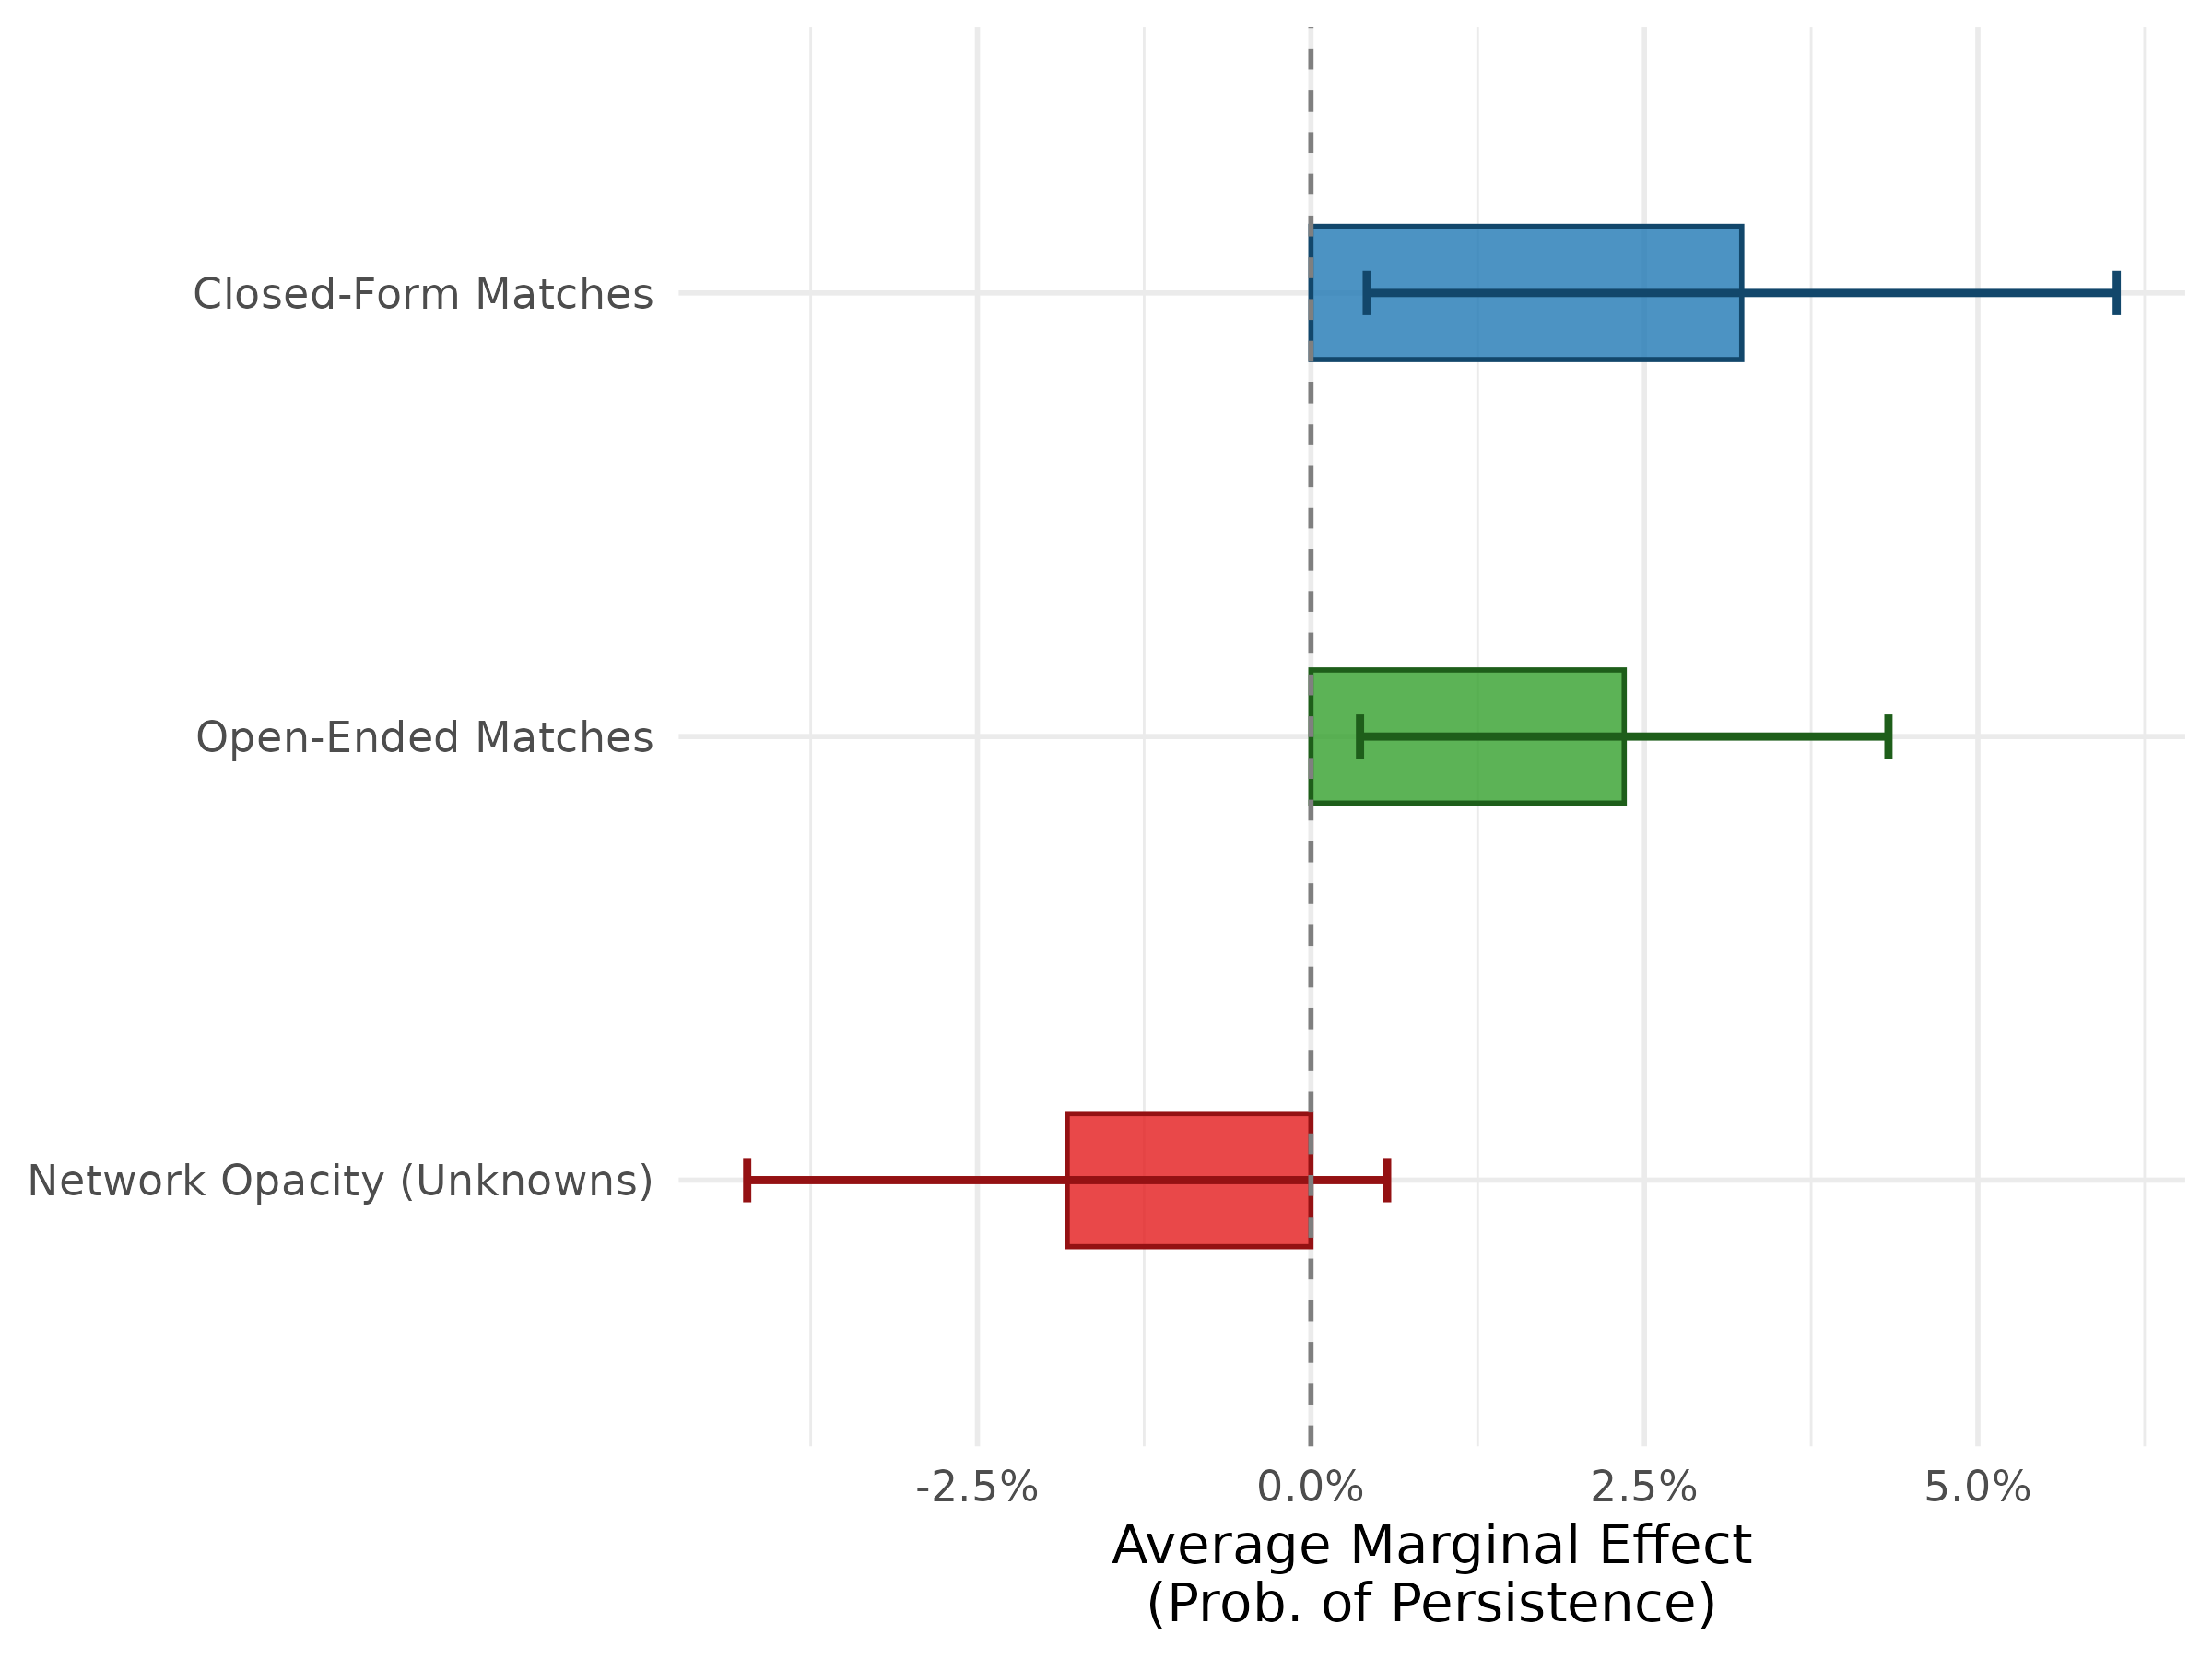
\includegraphics[width=\linewidth,keepaspectratio]{Plots/main_effects.png}
\caption{Predicted Probability of Protection from Tie Decay by Cultural Matching and Cultural Network Opacity.}\label{fig-combined}
\end{figure}

\newpage
\begin{figure}[htbp]
\centering
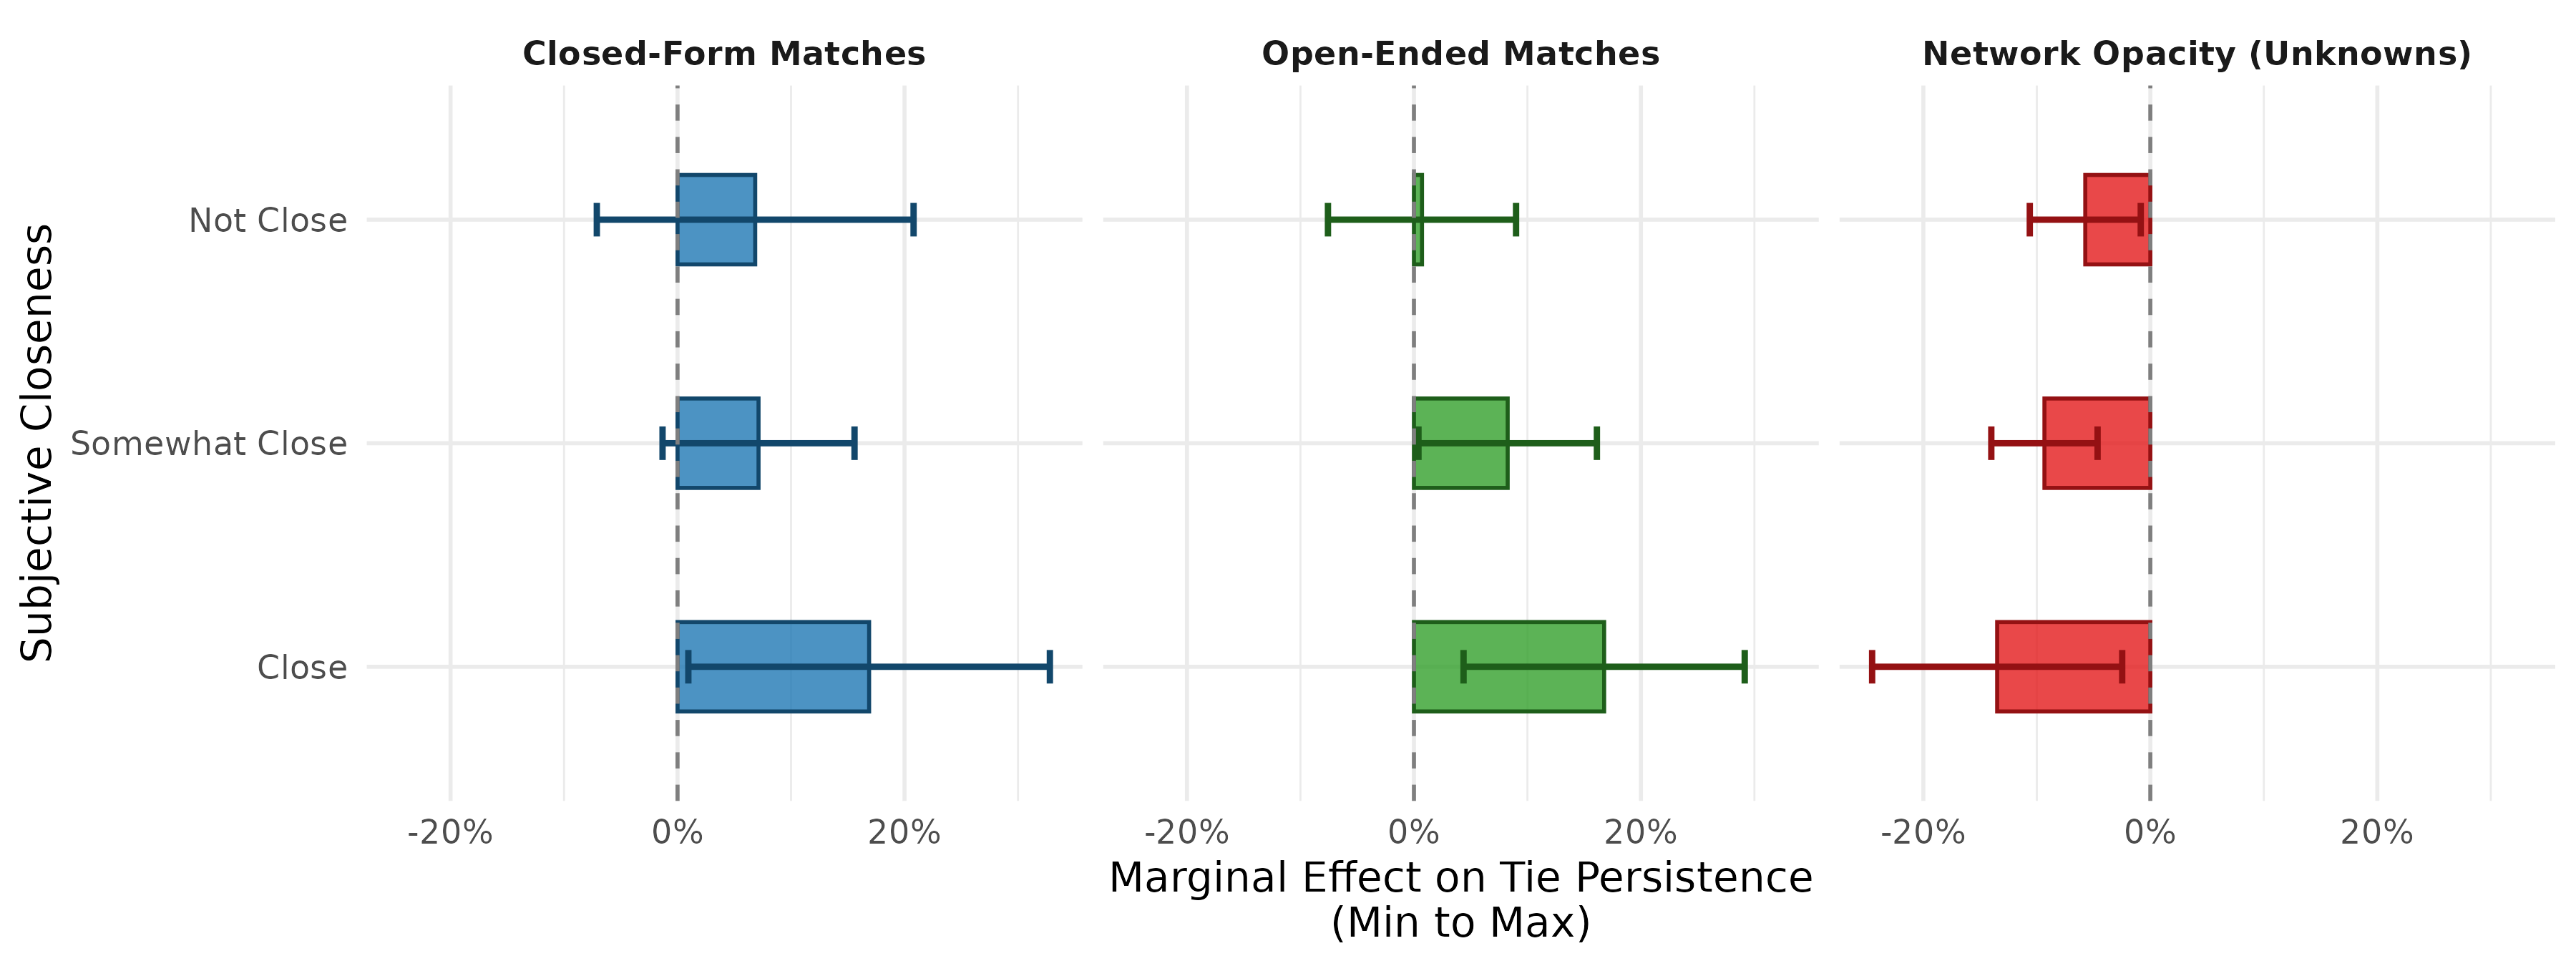
\includegraphics[width=\linewidth,keepaspectratio]{Plots/interaction_closeness.png}
\caption{Predicted Probability of Protection from Tie Decay by Cultural Matching, Cultural Network Opacity, and Subjective Closeness.}\label{fig-closeness-interactions}
\end{figure}

\newpage
\begin{figure}[htbp]
\centering
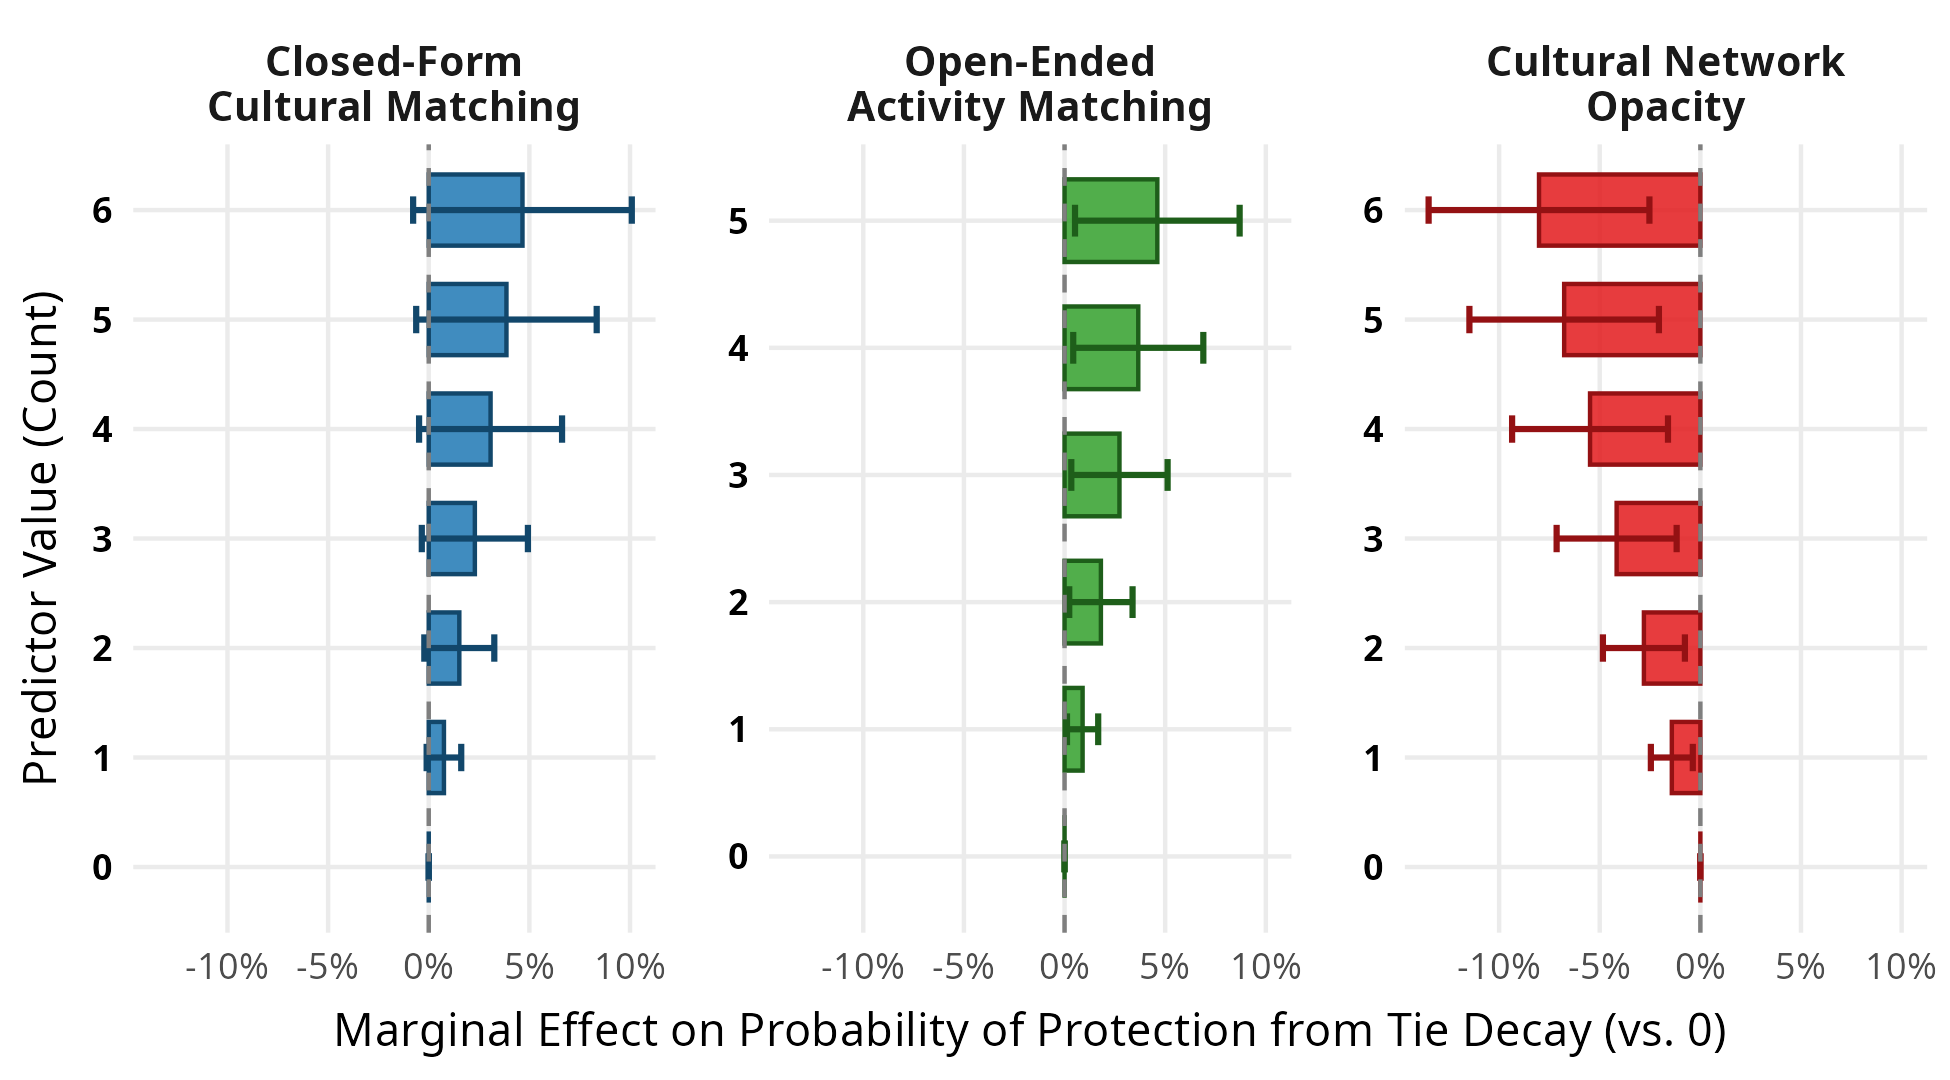
\includegraphics[width=\linewidth,keepaspectratio]{Plots/fe_predicted_probabilities.png}
\caption{Predicted Probability of Protection from Tie Decay from Ego Fixed-Effects Model.}\label{fig-fe-predictions}
\end{figure}


\clearpage

\bibliographystyle{apalike}
\sloppy
\bibliography{manuscript_citations}

\end{document}
